\section{Countermeasures optimization}

\subsection{Problematic}

\begin{frame}[fragile]{Countermeasures optimization approach} 
    \begin{small}
        \begin{itemize}
        \item Can some part of the countermeasure be removed without adding new attacks ?  
        \item[] $\Rightarrow$ Probl. P2 \& P4
        \item[] 
        \end{itemize}
        
        \onslide<1->{
            \begin{figure}[!ht]
            \centering
                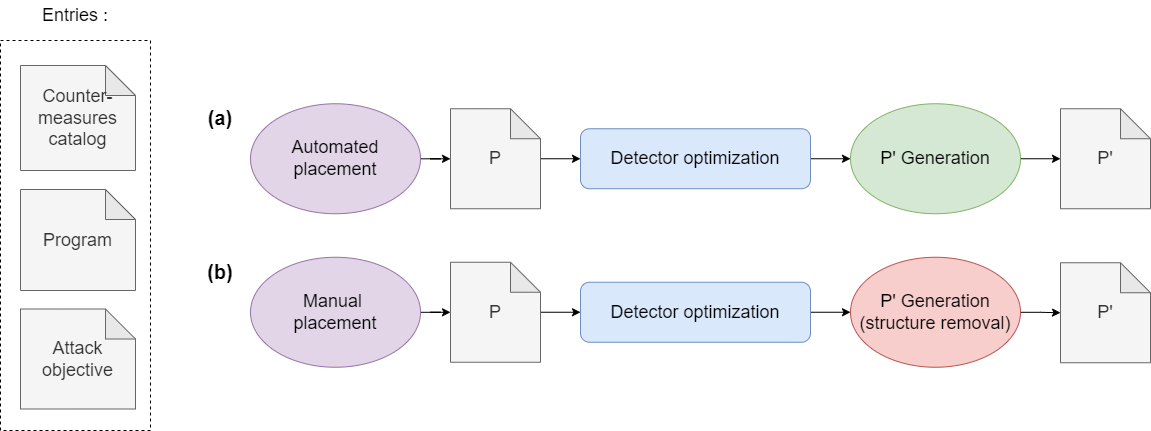
\includegraphics[scale=0.19]{img/placement-ccpo2-en.drawio.png}
                \label{fig:ccpo-metho}
            \end{figure}
        }
        
        \onslide<2->{
            \begin{itemize}
            \item[]
            \item \textbf{Approach:}
            \item[] $\Rightarrow$ focus on the subclass of detector-based countermeasures
            \item[] $\Rightarrow$ based on the execution with non-blocking detectors
            \end{itemize}
        }
    \end{small}
    \vfill
\end{frame}

\begin{frame}[fragile]{Definitions - Detectors and bodies} 
    \begin{small}
        \begin{columns}
            \begin{column}{0.5\textwidth}
                \begin{tiny}  
                    We divide a \textbf{detector-based countermeasure} in two parts:
                    \vspace{0.25cm}
                    
                    \begin{itemize}
                        \item {\color{RedViolet}Detectors} are control point in the program corresponding to sanity checks about the current state
                        \item The {\color{Bittersweet}countermeasure's bodies}: shadow variables, parameters, additional computation etc.
                    \end{itemize}
                    \vspace{0.2cm}
                    
                    \onslide<2->{
                         Examples
                         \begin{itemize}
                             \item \textit{Test duplication} (\textbf{TD}) 
                             \item \textit{Load Multiplication} (\textbf{LM})
                             \item \textit{SecSwift Control Flow} (\textbf{SSCF})\cite{Ferriere/LLVM19}: associates an unique identifier to each basic block and uses a xor-based mechanism to ensure that the correct branch has been taken
                             \item \textbf{LBH} \cite{Lalande/ESORICS14}: introduce step counters to protect against C-level instruction skips. Each counter verification is a \texttt{detector}
                         \end{itemize}
                    }
                \end{tiny}
            \end{column}
            \begin{column}{0.5\textwidth}
                \lstset{escapeinside={<@}{@>}}
                \lstset{style=customc}
                \begin{lstlisting}
bool compare(uchar* a1, uchar* a2,
    size_t size<@{\color{Bittersweet}, size\_t size\_dup}@>) {
    size_t i = 0u;
    bool result = true;
    <@{\color{Bittersweet}bool result\_dup = true;}@>
    
    for(; i < size; i++) {
        if(a1[i] != a2[i])
            result = false;
        <@{\color{Bittersweet}if(a1[i] != a2[i])}@>
            <@{\color{Bittersweet}result\_dup = false;}@> 
        
        <@{\color{RedViolet}if(result != result\_dup)}@>
            <@{\color{RedViolet}countermeasure();}@>
    }

    <@{\color{RedViolet}if(i != size)}@>
        <@{\color{RedViolet}countermeasure();}@>
    <@{\color{RedViolet}if(i != size\_dup)}@>
        <@{\color{RedViolet}countermeasure();}@>

    return result;
}
                \end{lstlisting}
            \end{column}
        \end{columns}
        \vspace{0.1cm}
    
        \textbf{Objectives}: 
        \begin{itemize}
            \item determine if some {\color{RedViolet}detector} could be removed, without adding any attack paths for the considered attack model.
        \end{itemize}
    \end{small}
\end{frame}


\subsection{Methodology}

\begin{frame}[fragile]{Countermeasure optimization - Idea: don't stop execution after detection } 
    \begin{tiny}
        \begin{itemize}
            \item Detector are considered as a structure \texttt{if(cond) killcard();} that can be attacked and \texttt{killcard} an atomic detection function
        \end{itemize}
        \onslide<2->{
            \begin{itemize}
                \item \textit{Intuition:} Explore the program executions by noting at each detector location if the corresponding detector would be triggered 
                \item[] $\Rightarrow$ all variation of detectors are considered in one single exploration.
                \item [] $\Rightarrow$ require side-effect free property on detectors
            \end{itemize}
        }
        \only<1>{
                \begin{figure}
                    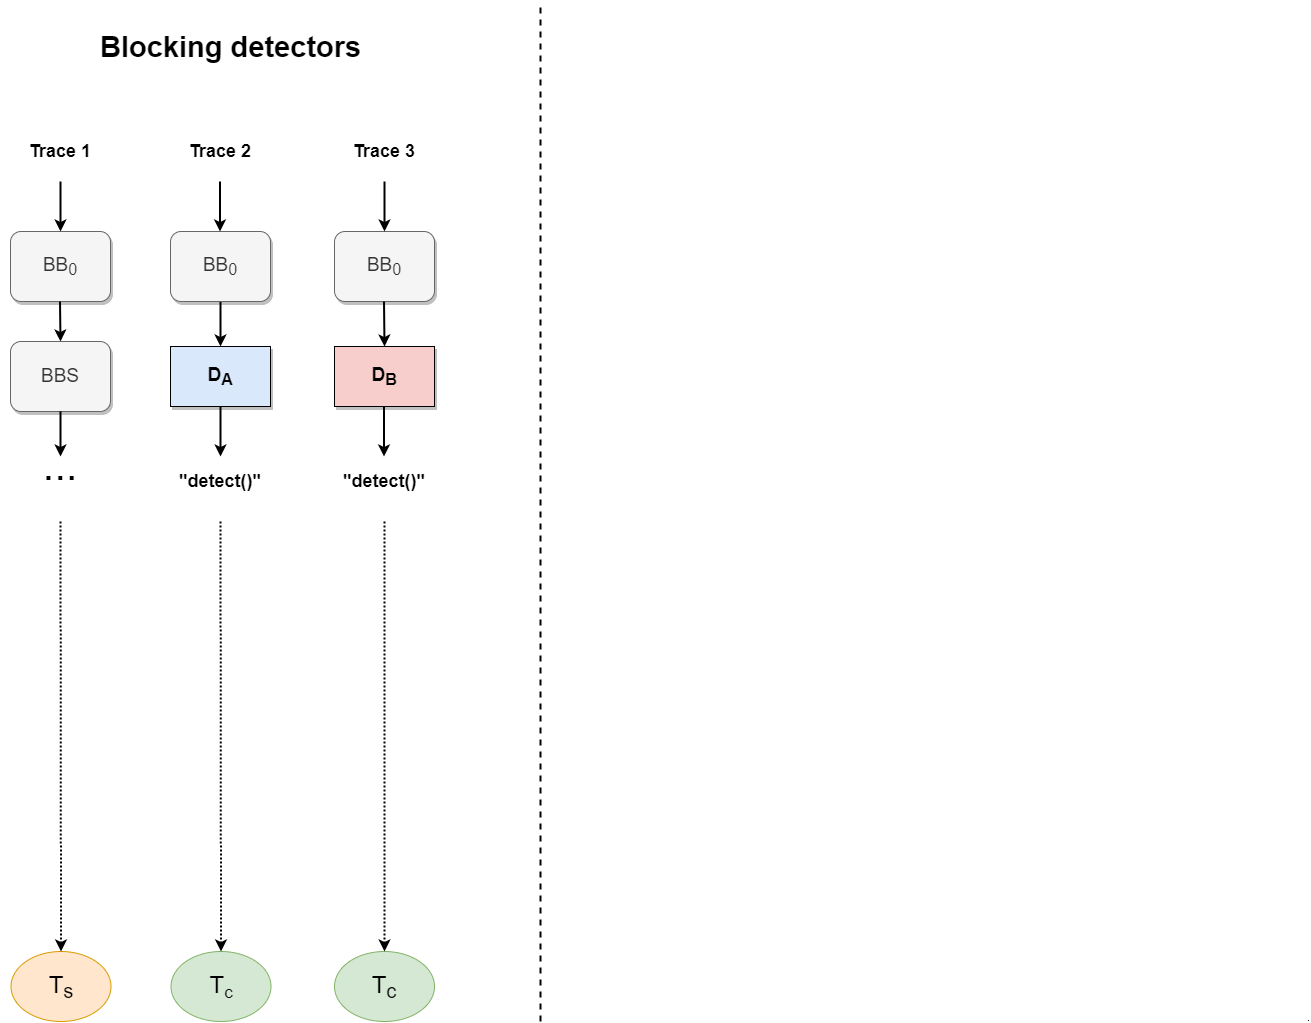
\includegraphics[scale=0.187]{img/CCP-prop-stopping2-simple.png}
                \end{figure}
        }
        \only<2>{
                \begin{figure}
                    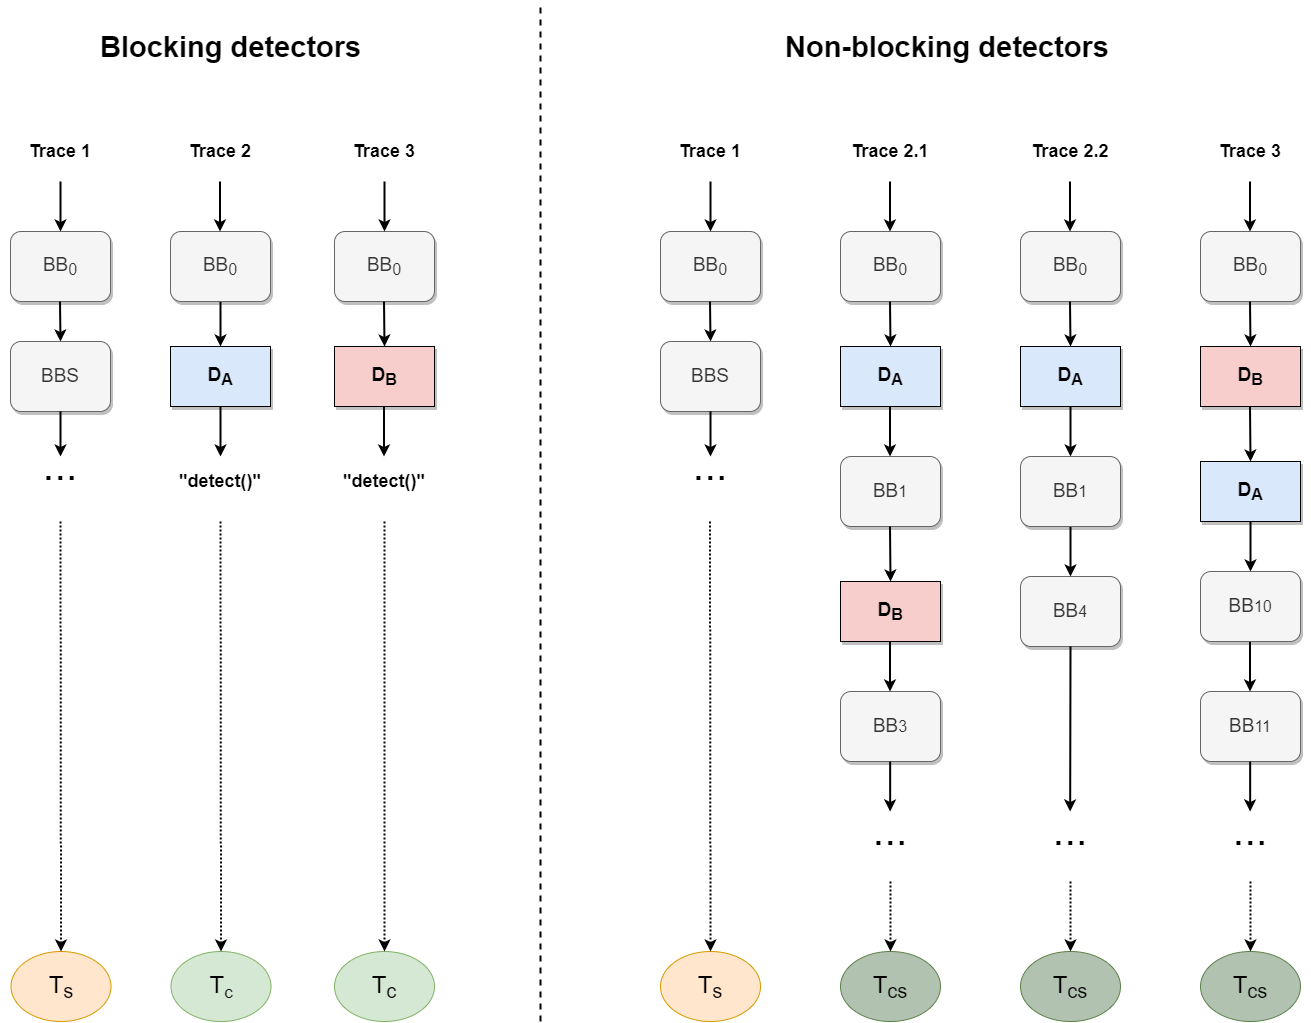
\includegraphics[scale=0.14]{img/CCP-prop-stopping2-en.drawio.png}
                \end{figure}
        }\only<3>{
                \begin{figure}
                    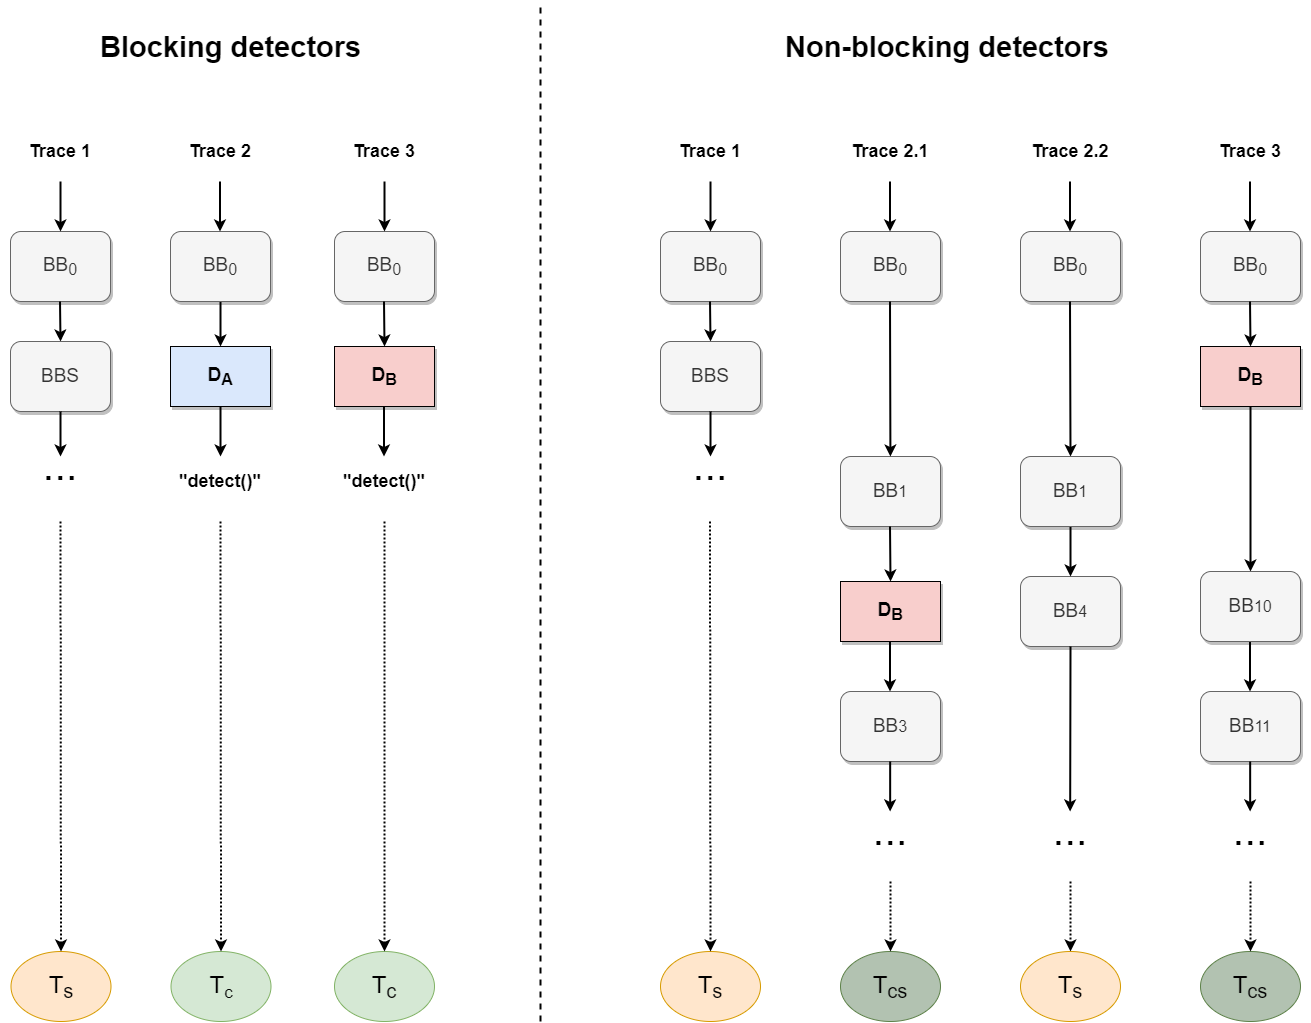
\includegraphics[scale=0.14]{img/CCP-prop-stopping2-en-DB.drawio.png}
                \end{figure}
        }\only<4>{
                \begin{figure}
                    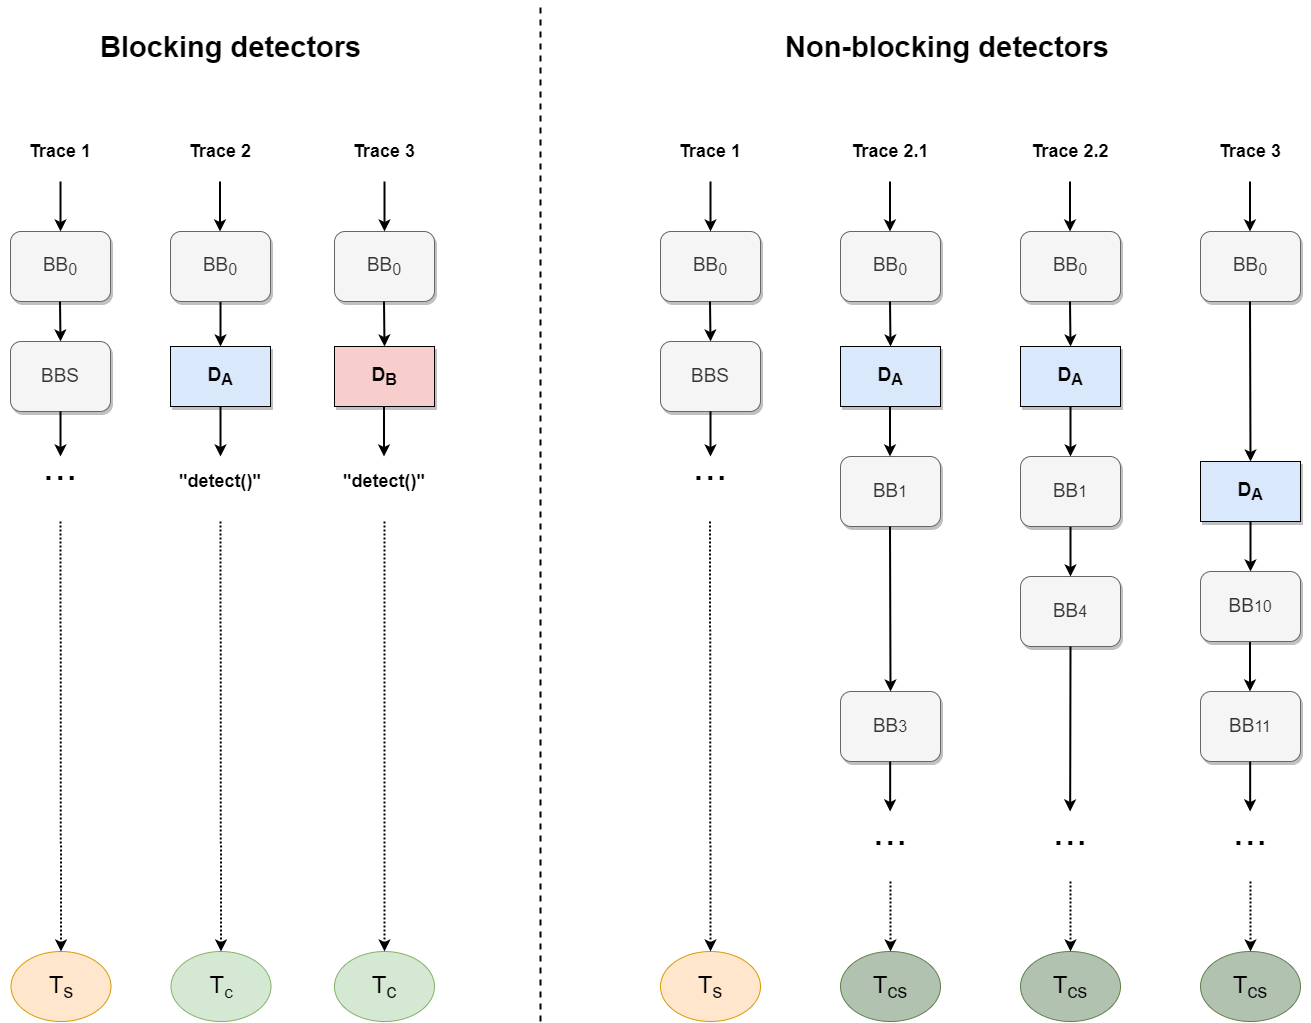
\includegraphics[scale=0.14]{img/CCP-prop-stopping2-en-DA.drawio.png}
                \end{figure}
        }
    \end{tiny}
\end{frame}

\begin{frame}[fragile]{Countermeasure optimization - Principle} 
    \begin{small}
        \begin{itemize}
            \item \textbf{An optimization problem:} Search the minimal set of detectors $\mathcal{D}$ such as at least one detector cover each trace of the set of detected attack traces
            \item[] $\Rightarrow$ using non-blocking detectors
            \item[] 
            \item[] 
            \item Exploration space can be reduced by \textit{classification} step:
            \begin{itemize}
                \item If $\forall t \in T', d_i \notin \{cm(t)\}$, $d_i$ is \textbf{inactive} (should be removed)
                \item If $\exists t \in T', cm(t) = \{d_i\}$, $d_i$ is \textbf{necessary} (should be kept)
                \item[] 
                \item Other detectors are \textbf{repetitive}
                \item[] $\Rightarrow$ focus on traces containing only \textbf{repetitive} detectors
            \end{itemize}
            \item[]            
        \end{itemize}
    \end{small}
\end{frame}

\begin{frame}[fragile]{Methodology - Step 1 - Test Duplication results in 2 faults}
    \textbf{VerifyPIN + Test Duplication:}
    \begin{itemize}
        \item[]
        \item 86 traces in 2 faults with \textbf{Lazart}
    \end{itemize}
    
    \begin{table}[]
        \caption{Detectors classification in 2 faults}
        \begin{tabular}{|l|l|l|l|l|l|l|l|l|l|l|l|}
            \hline
            \rowcolor[HTML]{C0C0C0} 
            Detector                           & 0 & 1                         & 2 & 3 & 4 & 5 & 6 & 7 & 8                         & 9                         & 100                       \\ \hline
            \rowcolor[HTML]{FFAC67} 
            \cellcolor[HTML]{C0C0C0}Class & R & \cellcolor[HTML]{FF8585}I & R & R & R & R & R & R & \cellcolor[HTML]{9AFF99}N & \cellcolor[HTML]{FF8585}I & \cellcolor[HTML]{9AFF99}N \\ \hline
        \end{tabular}
    \end{table}

    \begin{columns}
        \begin{column}{0.50\textwidth}
            \lstset{style=customc}
            \lstset{escapeinside={<@}{@>}}
            \begin{lstlisting}
bool verify_pin(uchar* user_pin) {
    if(try_counter > 0)      <@{\color{orange!80} \textbf{D0}}@> & <@{\color{red!80} \textbf{D1}}@>
        if(compare(user_pin, card_pin, PIN_SIZE)) {  <@{\color{OliveGreen} \textbf{D8}}@>
            try_counter = 3;
            return true;
        } else {  <@{\color{red!80} \textbf{D9}}@>
            try_counter--;
            return false;
        }
    return false;
}
            \end{lstlisting}
        \end{column}
        \begin{column}{0.5\textwidth}
            \lstset{style=customc}
            \lstset{escapeinside={<@}{@>}}
            \begin{lstlisting}  
bool compare(uchar* a1, uchar* a2, size_t size) {
    bool result = true;
    size_t i = 0;
    for(; i < size; i++) {  <@{\color{orange!80} \textbf{D2}}@> & <@{\color{orange!80} \textbf{D3}}@>
        if(a1[i] != a2[i]) {  <@{\color{orange!80} \textbf{D4}}@> & <@{\color{orange!80} \textbf{D5}}@>
            result = false; 
        }
    }

    if(i != size)  <@{\color{orange!80} \textbf{D6}}@> & <@{\color{orange!80} \textbf{D7}}@>
        countermeasure(100);  <@{\color{OliveGreen} \textbf{D100}}@>

    return result;
}
            \end{lstlisting}
    	\vfill
        \end{column}
    \end{columns}
\end{frame}

\begin{frame}[fragile]{Step 4 - Removed CCPs for verifyPIN (2 faults)}
	\vfill
    \begin{columns}
        \begin{column}{0.50\textwidth}
            \vspace{0.2cm}
            
            The {\color{Red}removed} and {\color{OliveGreen}kept} detectors and bodies for \textit{Test duplication} on \texttt{verify\_pin} with 2 faults
            \vspace{0.5cm}
    
            \lstset{style=customc}
            \lstset{escapeinside={<@}{@>}}
            \begin{lstlisting}
bool verify_pin(uchar* user_pin) {
    <@{\color{Red}bool c\_1;}@>
    <@{\color{OliveGreen}bool c\_2;}@>
    <@{\color{Blue}if}@>(<@{\color{Red}c\_1 = }@>try_counter > 0) {
        <@{\color{Red}if(!c\_1)}@>
            <@{\color{Red}killcard();}@>
            
        <@{\color{Blue}if}@>(<@{\color{OliveGreen}c\_2 = }@>compare(user_pin, card_pin, PIN_SIZE)) {
             <@{\color{OliveGreen}if(!c\_2)}@>
                <@{\color{OliveGreen}countermeasure();}@>
            try_counter = 3;
            <@{\color{Blue}return}@> true;
        } <@{\color{Blue}else}@> {
            <@{\color{Red}if(c\_2)}@>
                <@{\color{Red}countermeasure();}@>
            try_counter--;
            <@{\color{Blue}return}@> false;
        }
    } <@{\color{Red}else}@>
        <@{\color{Red}if(c\_1)}@>
            <@{\color{Red}countermeasure();}@>
    
    <@{\color{Blue}return}@> false;
}
            \end{lstlisting}
        \end{column}
        
        \begin{column}{0.5\textwidth}
            \lstset{style=customc}
            \lstset{escapeinside={<@}{@>}}
            \begin{lstlisting}
bool compare(uchar* a1, uchar* a2, size_t size) {
    bool result = true;
    <@{\color{Blue}size\_t}@> i = 0;
    <@{\color{OliveGreen}bool c\_1;}@>
    <@{\color{Red}bool c\_2;}@>
    <@{\color{Red}bool c\_3;}@>
    
    <@{\color{Blue}for}@>(; <@{\color{OliveGreen}c\_1 =}@> i < size; i++) { 
        <@{\color{Red}if(!c\_1)}@>
            <@{\color{Red}countermeasure();}@>
        <@{\color{Blue}if}@>(<@{\color{Red}c\_2 =}@> a1[i] != a2[i]) {
            <@{\color{Red}if(!c\_2)}@>
                <@{\color{Red}countermeasure();}@>
            result = false; 
        } <@{\color{Red}else}@>
            <@{\color{Red}if(c\_2)}@>
                <@{\color{Red}countermeasure();}@> 
    }
    <@{\color{OliveGreen}if(c\_1)}@>
        <@{\color{OliveGreen}countermeasure();}@>

    <@{\color{OliveGreen}if(}@><@{\color{Red}c\_3 = }@><@{\color{OliveGreen} i != size) \{}@>
        <@{\color{Red}if(!c\_3)}@>
            <@{\color{Red}countermeasure();}@>
        <@{\color{OliveGreen}countermeasure();}@>
    
    <@{\color{OliveGreen}\}}@> <@{\color{Red}else}@>
        <@{\color{Red}if(c\_3)}@>
           <@{\color{Red}countermeasure();}@>

    <@{\color{Blue}return}@> result;
}
            \end{lstlisting}
    	\vfill
        \end{column}
    \end{columns}
\end{frame}

\subsection{Experimentations}

\begin{frame}{Experimentations} 
    \begin{tiny}
        \begin{columns}
            \begin{column}{0.55\textwidth}
                \begin{table}[!t]
                    \centering
                    \label{tbl:ccpa-results}
                    \begin{tabular}{|l|c|c|c|c|}
                        \hline
                        Program       & \multicolumn{1}{l|}{Detectors} & \multicolumn{1}{l|}{1 attack} & \multicolumn{1}{l|}{2 attacks} & \multicolumn{1}{l|}{3 attacks} \\ \hline
                        VP + TD       & 11                       & 72\%                         & 63\%                          & 18\%                          \\ \hline
                        VP + SSCF     & 13                       & 92\%                         & 76\%                          & 23\%                          \\ \hline
                        VP + LBH       & 31                       & 93\%                         & 93\%                          & 32\%                          \\ \hline \hline
                        FU + TD       & 14                       & 0\%                          & 0\%                           & 0\%                           \\ \hline
                        FU + SSCF     & 24                       & 12\%                         & 12\%                          & 8\%                           \\ \hline \hline
                        GC1 + TD      & 39                       & 37\%                         & 34\%                          & 34\%                          \\ \hline
                        GC1 + SSCF    & 38                       & 57\%                         & 28\%                          & 28\%                          \\ \hline \hline
                        AES RK + TD   & 2                        & 50\%                        & 50\%                         & 0\%                         \\ \hline
                        AES RK + SSCF & 3                        & 66\%                        & 33\%                         & 0\%                         \\ \hline
                        AES C + TD    & 8                        & 50\%                         & 50\%                          & 0\%                           \\ \hline
                        AES C + SSCF  & 13                       & 76\%                         & 61\%                            & 38\%                             \\ \hline
                    \end{tabular}
                \end{table}
            \end{column}
        
            \begin{column}{0.5\textwidth}
                 Three countermeasures experimented:
                 \begin{itemize}
                     \item[]
                     \item \textit{Test duplication} (\textbf{TD}): presented previously
                     \item[]
                     \item \textit{SecSwift Control Flow} (\textbf{SSCF})\cite{Ferriere/LLVM19}: associates an unique identifier to each basic block and uses a xor-based mechanism to ensure that the correct branch has been taken
                     \item[]
                     \item \textbf{LBH} \cite{Lalande/ESORICS14}: introduce step counters to protect against C-level instruction skips. Each counter verification is a \texttt{detector}
                 \end{itemize}
            \end{column}
        \end{columns}
    \end{tiny}
\end{frame}